\chapter{研究内容}

\section{框架}
% 一页
针对城市中的各种交互问题,找到合适的研究尺度是给出解答的重点。在两个极端的尺度(即个体-微观,与整个城市的特征-宏观)之间,所有的尺度问题都可以用介观尺度的方法论加以解决。

第一个问题是针对问题的空间区域的提取。我们在利用地理大数据进行研究时,采样精度往往与需要探究的问题不完全一致,需要我们聚合成针对问题的合适尺度。比如,对于社会不平等的剥夺指数问题,研究数据主要是普查数据(普查范围是~8000人的无重合空间范围),而与之对应的政策调整范围则是更大的(区、县等数万人到数十万人的)区域。我们利用\textbf{扩散映射}技术,在多元数据中找到合适的参量,以针对需要的问题得到合适的空间范围。该方法不会从多元空间数据中选择特定的\textbf{列},而是从完整的数据集中构造一个针对问题的指标。由于其结构,扩散映射所提取的索引不会引入源数据偏见之外的偏见,并且对于数据操纵的企图具有很高的弹性。

第二个问题是介观尺度下的信息传播与共识达成问题。随着城市规模的增大,城市中各个区域的沟通也变得更加紧密。根据\cite{stark2008decelerating}, 更频繁的微观尺度交互会使得政策贯彻和城市面对外来冲击的弹性降低。为此,我们借鉴Hubbell模型\cite{hubbell2001unified},考虑不同社区中有若干个体,而每个个体针对一件时事(比如,疫情期间政府对于戴口罩的倡议)都有一个\textit{意见},在随机初始状态下意见统一的期望时间。我们发现,加入社区/集合种群等介观结构更容易达成意见统一。其他细致结构也对于我们理解介观结构对于形成城市意见共同体的影响。

第三个问题是介观尺度城市稳定性。城市各组分沟通得紧密也伴随着城市面临外在冲击时,冲击在城市内部快速的传导。城市面对流行病、战争等外来冲击时的抵抗能力通常被概括为城市韧性/稳定性。城市稳定性也对可持续发展的诸多方面(多样性,连通性,去中心化和自给自足)有解释作用。我们试图基于矩阵理论,利用城市中小区块的交互强度提出一种稳定性度量。在此理论下,可以通过求解矩阵的实部为负的特征值所占全部特征值的比例来衡量外来冲击在城市内部爆发的倾向性。

根据我们的理论和实证结果,介观空间单元的交互视角下,城市的空间连续性、一致性、稳定性等特征的结果都与微观尺度交互的结果不同。这说明城市中介观尺度观测结构不容忽视,是城市建模的重要一环。


\section{研究内容}
% 六七页

\subsection{利用扩散映射提取城市隐藏特征}

从认知、规划等角度来讲,城市空间都不是一个典型的欧氏空间:同样的欧氏距离下,穿不穿越河流、人流密集还是稀疏,都会产生不同的时间消耗和其他感知差异。这个事实说明城市空间的刻画是复杂的,全局的空间度量很难刻画城市空间的本质。为了更好的描述城市空间,我们需要更复杂的城市认知框架。数学上基于局部距离定义的\textit{流形}提供了一个可能的方案。

\begin{figure}
    \centering
    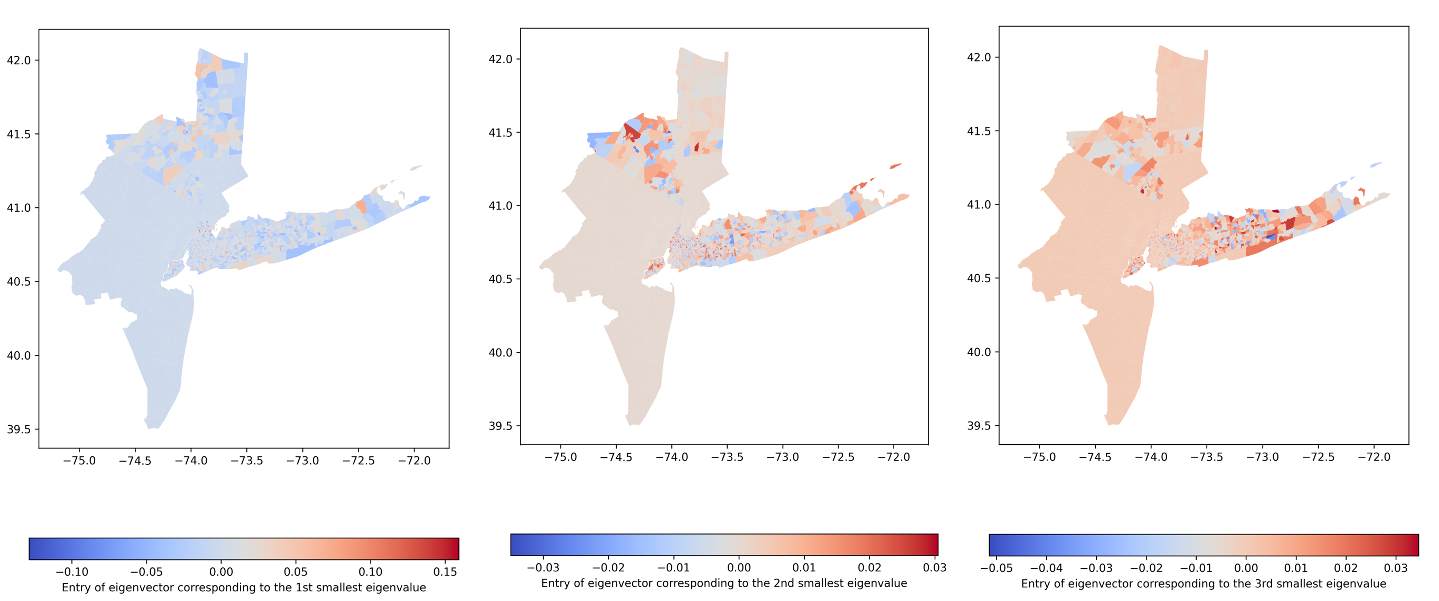
\includegraphics[width = 0.99\linewidth]{Figs/diffusionmap.png}
    \caption{扩散映射方法下,人口统计相关矩阵的前三小的正特征值对应的特征向量的空间分布。分别对应着纽约州的教育优势区域、贫困分布、和游客景点。}
    \label{fig:diffusionmap}
\end{figure}

Diffusionmap是一种流形学习方法。其出发点在于:很多多元数据的数据元只能反映客体的一部分特征,只有将多个条目的survey合起来才能得到一个比较完整的刻画。提取多个条目的survey的“权重”并不是一件简单的事,因为很多时候数据的特征是非线性变化的。这种特征往往很难用一种全局度量来衡量。流形强调的是局部性质:流形(Manifold)是局部具有欧式空间性质的空间,包括各种纬度的曲线曲面,例如球体、弯曲的平面等。流形的局部和欧式空间是同构的。流形学习假设所处理的数据点分布在嵌入于外维欧式空间的一个潜在的流形体上,或者说这些数据点可以构成这样一个潜在的流形体。流形是线性子空间的一种非线性推广。以英国的普查数据为例:英国在每个区域统计两类人口统计学指标:关键指标和快速指标。总共有1450个特征。\cite{barter2019manifold},作者用布里斯托及其周边的3490个人口统计学单元作为主要研究对象。其中的分析找到了解释统计反馈的主要变量:大学生密度和贫困程度。



\section{预期创新点}

本文通过引入较多的数学工具,对城市介观尺度下空间模式的提取、交互模式的性质、局部模式的涌现进行研究。本文的几个主要结果改进了地理大数据采集的设计,提出了定量衡量城市政策效果的方法,证明了介观尺度模式涌现的必然性。预期创新点如下:\begin{enumerate}
    \item 改进扩散映射方法,引入负相似性的概念
\end{enumerate}